\section{The Manifold High-Level Language}

\subsection{Module System}

Designing a microfluidic circuit requires common components to be made available to the user in the 
form of libraries. To facilitate code reuse and sharing we created a basic module system for Manifold.
The standard libraries for each domain will define APIs for interacting with the corresponding Manifold
backend. We are currently developing such a library for the microfluidics backend. The Manifold libraries
define \texttt{primitive nodes} that a backend will later recognize as components. These basic
components would be very difficult or impossible to represent natively in Manifold,
so instead we simply define an interface for the backend library. Creating
modules in Manifold also allows users to share their circuit designs and have
others build on them, a practice that is common in microfluidics.

The module system new in Manifold 2.0 supports the essential functionality required by a module system,
as outlined by Cardelli \cite{Cardelli:1997:PFL:263699.263735}. These
essential features are described in the rest of this section. Each module, in this case a file, can
declare functions and values as \texttt{public} --- the exports. When a module imports another
module all of the exported values in the imported module will be
accessible. Other programming languages, such as Simple ML, feature more exotic module systems, but this
additional complexity is not currently beneficial to Manifold. \autoref{lst:exports} shows a module
that exports several values, as well two
fluid nodes that use \texttt{Nil} to denote no input or output.

\begin{lstlisting}[label=lst:exports, caption=Exported values in a Manifold file]
public microfluidPort = primitive port Bool;

public tJunction = primitive node (dispersed: microfluidPort, continuous: microfluidPort) -> (output: microfluidPort);
public fluidEntry = primitive node (viscosity: Real) -> (output: microfluidPort);
public fluidExit = primitive node (input: microfluidPort) -> (Nil);

// Constant that is not exported
MIN_CHANNEL_SIZE = 0.0001;
\end{lstlisting}

On import, all exported values are returned by the import
expression. In Manifold all language constructs are
expressions, and imports are no exception. This differs from how imports are
treated as statements in many other
programming languages, even in other functional languages like Haskell and
OCaml, imports do not return a value.  Import expressions allow the
exported values of a module to be scoped by assigning the result of the expression
to a variable. The imported values are then referenced as properties of that
variable, see \autoref{lst:imports}. A module effectively becomes, and is used as,
a record data type. Manifold's import style is similar to a module syntax for Scheme proposed by
Curtis and Rauen \cite{Curtis:1990:MSS:91556.91573}. Their module system used
a function called \texttt{access} to reference the values exported by another
module. They also proposed a function called \texttt{open} that would reduce
the verbosity of qualifying access to a module's exported values, by adding the
argument's exported values to the current lexical scope. Manifold does not
have a similar construct.

\begin{lstlisting}[label=lst:imports, caption=A module imported into a Manifold file]
mf = import "microfluidics";
mf::microfluidPort in = mf.entryPort(viscosity=2.0);
\end{lstlisting}

\subsection{Type System}

Many user errors in Manifold 1.0 resulted in errors during backend compilation. It is very difficult
to determine what the source of the problem was when an error is discovered this late in the compilation
process. Manifold 2.0 includes a static type checking system to increase the percentage of bugs found during
the compilation stage, when more information can be communicated to the user about their error.
Similar to typedefs in the C programming language, Manifold allows users to define and import type aliases.
Variables can also be annotated with a specific type. Upon compilation,
Manifold performs static type checking on all expressions, inferring the type of a variable when it
is not explicitly defined.

The type system demonstrated in \autoref{lst:types} is Manifold 2.0's structural typing system.
Structural type systems were
created to remove some of the issues with nominal type systems
\cite{Gil:2008:WIS:1449764.1449771}. In a structural
type system, a type A is compatible with another type B if for every feature in
A there is a compatible feature in B. Unlike nominal type systems, structural
type systems allow for sub and supertypes to be defined without
modifying the original type. This allows for complex derived types in Manifold that
can extend the provided standard libraries.

Manifold allows the assignment of subtype values to a variable declared with a supertype of that value,
but not vice-versa.
However, tuple types are the exception to this rule. Tuples are
considered compatible if the signatures of two tuples
match by comparing the fields of the tuples.
Some structural typing systems will allow assignment to a type with a subset of the source's fields.
In Manifold, tuples are often used to describe components, and we expect it will usually be a logical error to allow
fields of a component be lost in a cast. As a result, this feature of structural typing is omitted to
prevent user errors.

\begin{lstlisting}[label=lst:types,caption=Example of types in a Manifold file]
// Type definitions
Type Fluid = Int;
Type Pump = (f: Fluid, control: (on: Bool));
Type DoublePump = (first: Pump, second: Pump);

// Variable declarations
DoublePump p;

// Basic structural typing
p1 = (fluid=1, control=(on=true));
(fluid: Int, control: (on: Bool)) p2 = p1;
p2 = (first=p1, second=p2);
\end{lstlisting}

% TODO:
% Compared to <insert similar type systems>, Manifold differs in its approach. Explain how
% Maybe list a feature (potentially from one of the other type systems compared) we want to add to Manifold in the future

\subsection{Improvements to Tuples}

Other work on the Manifold language was dedicated to improving the programmer's experience of using
tuples in Manifold. Tuples are used extensively in Manifold and their
fields could previously only be accessed using numeric indices. This was not
semantically meaningful to a user, and made the usage of tuples confusing. One way we improved the usage of tuples
was by extending
Manifold with the ability to unpack tuple fields. Unpacking of a tuple's
fields is a common feature of functional programming languages, and involves declaring
variables using a tuple on the left-hand side of an assignment expression. We
also added named fields to tuples, inspired by Python's \texttt{NamedTuple}
class. Naming fields means that a programmer can refer to a field of a tuple using an
index or the name of that field. Named fields increase the readability of
Manifold and helps users of the language coming from languages like C that offer this functionality
with structs or a similar data type. The new tuple language features are shown in \autoref{lst:unpacking}.

\begin{lstlisting}[label=lst:unpacking, caption=Examples of new tuple features]
mf = import "microfluidics";

// Use unpacking to do parallel assignment
(waterViscosity, oilViscosity) = (1.002, 250.0);

makeTJunction = (Nil) -> (output: mf::microfluidPort, dispersed: mf::microfluidPort, continuous: mf::microfluidPort) {
  continuous = mf.fluidEntry(viscosity=waterViscosity);
  dispersed = mf.fluidEntry(viscosity=oilViscosity);
  output = mf.tJunction(output=output, dispersed=dispersed, continuous=continuous);
};

tJunctionChannels = makeTJunction();
// Access a field on the return value using the named attribute
mf.fluidExit(tJunctionChannels.output);
\end{lstlisting}

\section{The Manifold Microfluidics Backend}

\subsection{Modelica Code Generation and MapleSim Integration}

Modelica is an open-source and multi-domain modelling language that can be used
to create and simulate models of a system. \cite{Maplesim}\cite{modelica}
Manifold 1.0's SMT2 code generation and dReal integration are suitable for
determining a system's basic viability, but the techniques are insufficient for
analysis in greater depth.
A list of SMT2 equations can be evaluated for the basic feasibility of a system, but they do not create
a complete model of the system.
Generating Modelica code was of interest to circuit designers because it allows the backend to create simulations of the
synthesized model.
Modelica models are more expressive than SMT2 equations and can simulate how the system will behave with time.

Modelica is an open standard, and there are many software frontends that support it.
We chose to integrate Manifold with MapleSim, a proprietary simulator developed by MapleSoft.
MapleSim offers a Java API called OpenMaple, allowing it to be called programmatically by Manifold.

Modelica models for MapleSim are straightforward to generate from a Manifold schematic.
A MapleSim model is a list of design components that are connected to each other using their ports.
The Manifold schematic format also has concepts of nodes, ports, and connections, allowing a simple mapping
between the two formats.
% TODO(nik): What is CAD, can we explain this acronym?
To identify the type of a component, the Manifold microfluidics backend relies on the attributes of the nodes.
On top of the core Modelica code, MapleSim supports annotations that specify the positions of components on a CAD interface and the settings of the simulations.
The Manifold microfluidics backend usually cannot infer the values of these annotations from the schematics
alone and instead tries to fill in the values with reasonable defaults.

A Modelica model can list components and their types (e.g. rectangular pipes, T-junctions, fluid exit points),
but it does not contain specific domain knowledge or physical equations that describe how exactly these
component works.
Instead, the inner workings of components are specified in libraries.
MapleSim has libraries with equations for components in domains fields such as hydraulics and electrical
circuits, both of which have some analogies to microfluidic circuits.
A specialized microfluidics library for MapleSim is currently under development at the University of Waterloo
in collaboration with the Manifold team.

We have not yet leveraged Modelica code generation for microfluidics because of a lack of a sufficient
MapleSim library, however, once the models are developed integration with Manifold will be straightforward.
MapleSim representations for simple fluid components such as rectangular pipes exist, but models of more complex components such as T-junctions are still in progress.
We have demonstrated the viability of the Manifold's backend to generate Modelica code by using
libraries from different domains, such as hydraulics and electrical circuits. Our results for the Modelica
code generation and simulation of a rectangular pipe are shown in \autoref{fig:pipe-schematic} and
\autoref{fig:pipe-simulation}, respectively.

\begin{figure}[!ht]
  \caption{MapleSim schematic of a simple rectangular pipe}
  \centering
    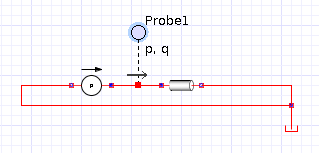
\includegraphics[width=0.5\textwidth]{img/simple-pipe.png}
	\label{fig:pipe-schematic}
\end{figure}
\begin{figure}[!ht]
  \caption{MapleSim simulation of a simple rectangular pipe}
  \centering
    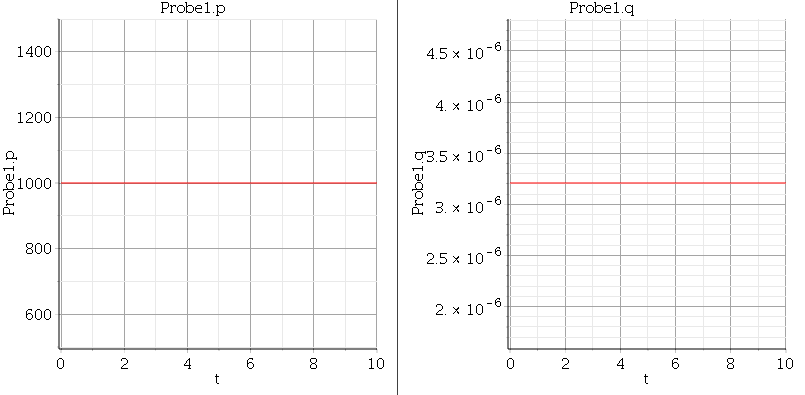
\includegraphics[width=0.5\textwidth]{img/simple-pipe-simulation.png}
	\label{fig:pipe-simulation}
\end{figure}

\subsection{Inferencing with Incomplete Descriptions}

With Manifold's existing SMT2 code generation, engineers can specify all the
relevant details of their microfluidic devices and delegate determining if the system is viable to Manifold. When engineers
are unsure of a value using the current methodologies they make a guess and manually check its
validity. A common engineering use case is that the engineer is unsure of the
values of one or more design parameters and is interested in finding an
acceptable range. To accommodate this workflow, Manifold now allows certain
attribute values to be left unspecified, and it becomes the
responsibility of the backend to find a suitable value.

Manifold 2.0 allows designers to opt out of
specifying a value for an attribute using the value {\tt infer} instead of a
concrete value. Inferred values are noted in the intermediate schematics as
being inferred so that a Manifold backend can recognize that there is a missing value.
By the end of a successful run, the backend will have populated all inferred variables with values.

The microfluidics backend begins the process of resolving inferred values by generating SMT2 equations
and querying dReal for a solution.
If dReal returns that the system of equations is unsatisfiable, Manifold notifies the
user and asks the user to change the design. If dReal is unable to prove the system of equations is unsatisfiable,
it outputs a range of values for the inferred variables to be further tested.
The microfluidics backend parses the dReal outputs and chooses values within the given ranges for the
unspecified variables.
The process of choosing an acceptable value from within the range given by dReal is still a matter of
guessing, and a more sophisticated algorithm would offer a beneficial improvement over a random search.
Once values have been assigned to all the inferred variables in the schematic, the backend generates Modelica code.
The backend invokes MapleSim using the OpenMaple API to simulate the behaviour of the generated models.
If the simulation is not successful, the backend can select different values for the inferred variables
and reattempt the simulation.

\section{Related Work}

Manifold inherits from the mature research area in software engineering of
design automation and hardware description languages. Automated synthesis of VLSI has had
significant contribution to the development of silicon devices over the last few decades
\cite{MeadConway80}. There has been some work on automated synthesis in the area of microfluidics.
\emph{MHDL}, for example, is a language for describing microfluidic circuits in a modular way, and the
synthesis program treats the microfluidic circuit similar to an FPGA \cite{McDaniel13aspdac}. The
expressiveness of Manifold is more generic than that of MHDL, and the underlying complexity behind
the components is hidden from the programmer in the domain specific backends. The introductory
publication of Manifold \cite{Berzish16cascon}, has more citations of related work in the domain of
microfluidics.

In the realm of synthesis, a new paradigm in design automation is ``Approximate hardware design''.
Axilog is a tool introduced in \cite{axilog}, which describes a procedure for approximating design
parameters using relaxibility inference analysis. This is different from Manifold's synthesis
framework because the synthesis in Manifold happens using dReal, which is a combinatorial approach
of equation solving using boolean satisfiability. In contrast, Axilog employs an algorithmic and
interactive optimization technique for synthesis.

\section{Future Work}

\subsection{Manifold Language}

Microfluidic circuits often have identical components that are used repeatedly.
We would like to add looping constructs to Manifold, either by creating a
macro system or by creating built-in Manifold functions. A looping function
would take a component as a parameter and then repeat an action on that
component a number of times, such as connecting it to other components.
This feature in Manifold would not only prevent the programmer from repeating
code, but would also allow a programmer's design to scale up to a number of
components that would not be feasible to write by hand. We also intend for
programmers to be able to specify parameters for components, such as a T-junction with \emph{n} branches.

\subsection{CEGAR Loop}

The Manifold backend's toolchain flow has so far been entirely linear.
The verification workflow is only run once and the simulation results from MapleSim are returned
to the programmer, not evaluated by Manifold. This workflow can be enhanced by creating a feedback
loop.
By interpreting MapleSim's outputs, the Manifold backend can determine how successful the simulation was
relative to the engineer's requirements.
Based on these results, the backend would revisit the systems of SMT2 equations it generated earlier.
New values from within dReal's output ranges could be chosen for the next MapleSim generation.
This process will be repeated until the validity of the system is certain to within a desired threshold.
Another way the MapleSim results can be used is in constraining the values of inferred parameters to
smaller ranges, and running dReal again on the increasingly constrained system.

This process is called a CEGAR loop. CEGAR stands for ``counterexample-guided abstraction refinement'' \cite
{cegar}.
The principle is that when a system fails a satisfiability test or simulation, the failed system
serves as an example of what a successful system is not.
The counterexample helps reduce the plausible ranges for the system parameters.
Given enough runs of a CEGAR loop, the ranges of inferred variables is within a margin that a prototype
can feasibly be built.

\subsection{COMSOL Code Generation}

COMSOL Multiphysics (``COMSOL") \cite{comsol} is a powerful and proprietary simulator and finite element analyzer \cite{fem}.
It supports add-ons for a wide variety of domains, including fluid mechanics.
We are interested in applying COMSOL because it promises a more deep and thorough simulation of the microfluidic devices than what MapleSim is capable of.
COMSOL has a Java API, so it should be possible to integrate it into Manifold's existing Java codebase and have it be called automatically.

We would like to add COMSOL simulation as another verification step to be run after the CEGAR
loop described previously.
COMSOL is much slower and much more thorough than dReal or MapleSim, so it is impractical to include
in the main analysis loop. However, a COMSOL simulation would give a much higher degree of confidence in the
validity of a design.
